\section{Introduction}
The COVID-19 pandemic, as a global public health crisis, has precipitated unprecedented societal, economic, and political disruptions, underscoring the imperative of real-time epidemic forecasting. However, many of the epidemic surveillance values published by public health surveillance data systems are often and repeatedly revised in subsequent releases after their first release, and do not accurately reflect disease activity in real time. This often leads to biased and error-prone situational awareness\cite{McGough2020}\cite{Rosenfeld2021} and poses substantial hurdles to achieving real-time epidemic forecast accuracy.

The impact of reporting delays and subsequent data revisions has been discussed not only in the context of public health studies: from influenza\cite{chakraborty2018know} to dengue \cite{rangarajan2019forecasting} to COVID-19 forecasting\cite{rodriguez2021deepcovid}\cite{adiga2020mathematical}, but also in the macroeconomic domain\cite{clements2019data}. Data revisions arise from various factors, including error corrections, infrastructure limitations, and varying delays between data collection and reporting\cite{reich2019collaborative}\cite{Chakraborty2018}. These factors affect surveillance values differently, leading to distinct data revision patterns. For example, case counts typically increase monotonically during the revision process, a phenomenon commonly referred to as "backfill.". However, epidemic fractions (e.g., the percentage of positive COVID-19 insurance claims out of total claims) often fluctuate—either increasing or decreasing—dramatically due to different backfill dynamics of the numerator and denominator.

Several studies have addressed data revision and reporting delay issues, particularly in the context of seasonal infectious diseases with extensive weekly surveillance data. Early approaches relied on relatively simple statistical models. For instance, linear regression was used to adjust provisional data and forecast ILI case counts across 15 Latin American countries \cite{chakraborty2014forecasting}, while the residual density method was applied to estimate the distribution of revised updates in weekly ILI data \cite{brooks2018nonmechanistic}. More recent efforts have focused on probabilistic and Bayesian frameworks to better handle uncertainty and temporal variation in delays. A flexible Bayesian model, Nowcasting by Bayesian Smoothing (NobBS), was introduced to accommodate time-varying delay distributions and improve uncertainty quantification for dengue and ILI case counts \cite{McGough2020}. Generalized Bayesian methods using Laplace approximation were applied to dengue and SARI data in Brazil \cite{bastos2019modelling}, and a generalized Dirichlet-multinomial mixture model was proposed for weekly dengue data in Rio de Janeiro \cite{stoner2020multivariate}. Other approaches have incorporated structured or semi-mechanistic models; for example, nowcasting delayed norovirus cases in England during winter 2023/24 has been tackled using generalized additive models, Bayesian structural time series, and Epinowcast \cite{van2019nowcasting, epinowcast}. Some models also account for backfill uncertainty without explicitly modeling its dynamics \cite{osthus2019even}.

Comparatively, while COVID-19 surveillance data provide finer temporal granularity through the shift from weekly to daily reporting, they are considerably noisier and less regular than surveillance data for seasonal infectious diseases. This added variability complicates the extraction of stable features needed to characterize revision patterns. To address these challenges, several recent methods have been proposed. A neural network-based framework has been proposed to refine COVID-19 forecasts using weekly case counts~\cite{kamarthi2021back2future}. Although effective, this method requires substantial computational resources and does not account for the statistical properties inherent in public health datasets. Besides, a Bayesian spatiotemporal nowcasting model was introduced to estimate COVID-19 case counts at the county level in Ohio, incorporating an autoregressive structure to capture temporal dynamics~\cite{kline2022bayesian}. Both methods focus exclusively on count-type data and were evaluated only during the pre-Delta phase of the pandemic.

Among existing methods, Epinowcast\cite{epinowcast} stands out as a strong competitor leveraging a full Bayesian framework for nowcasting with robust uncertainty quantification. However, the reliance on Bayesian inference makes it computationally intensive, often requiring long runtimes, which can limit real-time applicability. Furthermore, Epinowcast and similar Bayesian models are designed primarily for count-type data and are less adaptable to fraction-type quantities. This presents a notable limitation, as many important public health indicators—such as antigen test positivity rates, hospitalization ratios, and syndromic surveillance measures—are expressed as fractions rather than raw counts. This limitation arises from the fact that Bayesian methods are generally built on assumptions of an underlying mechanistic process for how count data evolve over time, an assumption that does not hold for many fraction-type data, which often lack a clear generative structure.

In the broader forecasting literature, data revisions and real-time analysis have been extensively studied in macroeconomics. Notably, comprehensive surveys have been conducted on these topics~\cite{croushore2006forecasting, croushore2011forecasting}, and various modeling approaches—such as state-space models—have been summarized~\cite{clements2019data}. However, these macroeconomic methods are not directly transferable to public health contexts. Revisions in public health data are driven by health-seeking behavior and the administrative practices of public health agencies which are influenced by operational constraints, staffing capacity, and evolving reporting protocols.

In this paper, we focus on the distributional forecasting of finalized surveillance values in \textit{real time}. We introduce Delphi Revision Forecast (Delphi-RF), a robust and operational framework for correcting data revisions, which is openly available at https://github.com/cmu-delphi/DelphiRF. Delphi-RF is designed to handle signals with varying temporal resolutions and is applicable to both count-type and fraction-type data. When estimating quantities relative to a given estimation date $s$, our approach ensures that only data available up to that date are used. Specifically, the correction system uses all revisions recorded up to $s$ to estimate the probability distribution of the finalized values, which become fully available only at a later stage.

The Delphi Group at Carnegie Mellon University curates real time infectious disease indicators and makes them accessible via public API\cite{reinhart2021open, mcdonald2021can, farrow2015delphi}. When applied to a variety of such indicators, we have shown that Delphi-RF provides competitive or superior forecast accuracy for data revisions, including for COVID-19, dengue fever, and ILI. Moreover, Delphi-RF achieves an over 10- to 100-fold improvement in computational efficiency compared to existing methods, making it a scalable and practical solution for real-time public health surveillance.

The remainder of this paper is structured as follows. Section 2 introduces the problem formulation, along with key terminology and notation. Section 3 details the proposed model, the evaluation framework, and the adaptive modeling protocol. Section 4 describes the datasets, preprocessing steps, and experimental setup, followed by results demonstrating the model’s performance across multiple COVID-19 indicators, as well as comparative analyses with alternative methods applied to other infectious diseases. Finally, Section 5 concludes with a discussion of the findings and outlines directions for future research.

\begin{figure}[h!]
    \centering
    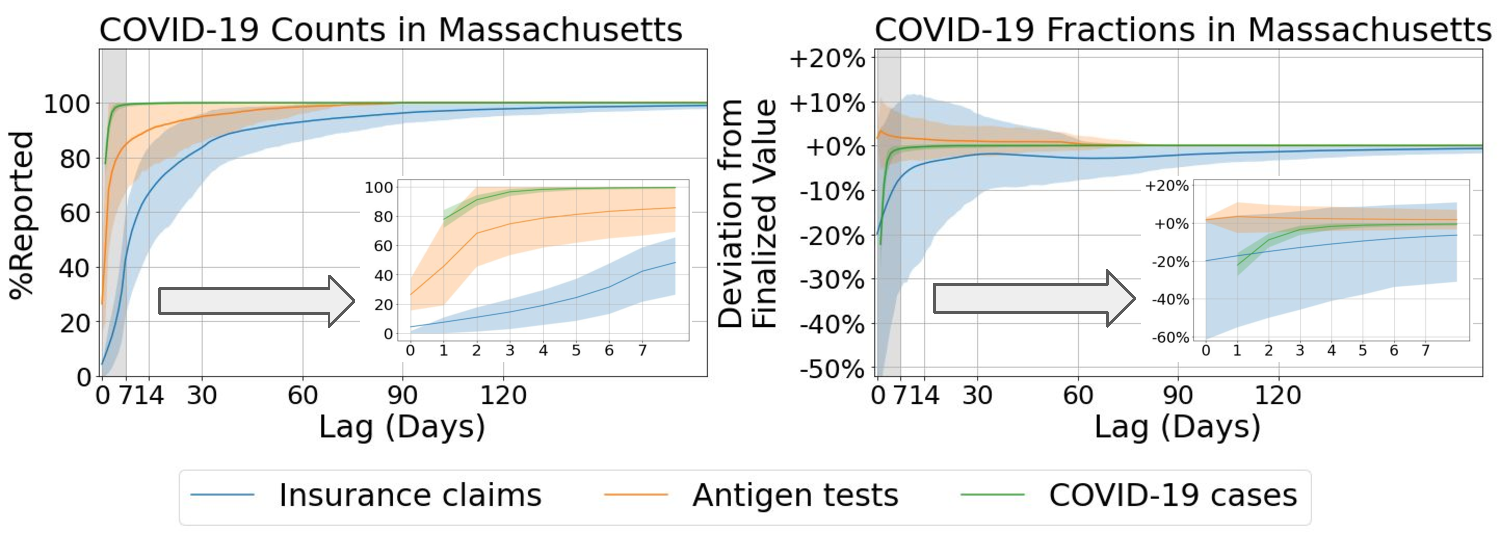
\includegraphics[width=\textwidth]{figs/Intro_fig.pdf}
    \caption{\textit{\textbf{Data revision patterns for different indicators.} Left: Mean percentage of counts reported relative to the values revised 300 days later, averaged over all reference dates and plotted by reporting lag for Massachusetts. Shaded bands represent the 10th to 90th percentile interval. Right: Mean values of COVID-19-related fractions normalized by their corresponding revised values after 300 days, also averaged over all reference dates and plotted by lag for Massachusetts.}}

\end{figure}



